\begin{figure}[h]
    \centering
    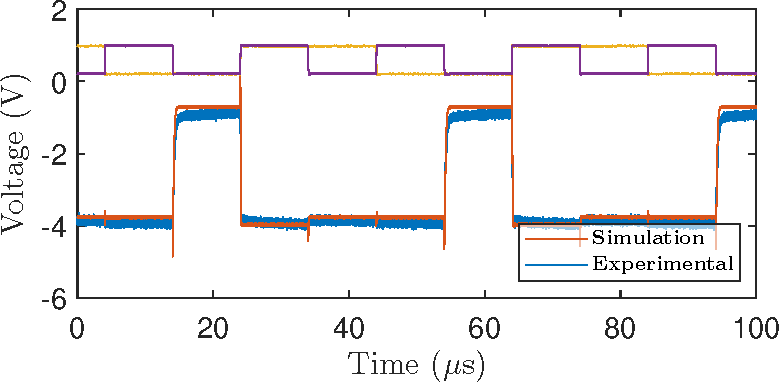
\includegraphics[width=1\linewidth, height = 5.1cm]{Appendices/NOR50K.pdf}
    \caption{Experimental and simulated NOR gate output voltage at 50 kHz Shifted by 1.5 V. The gate input voltages have been scaled and offset to the top of the diagram.}
    \label{fig:enter-label}
\end{figure}

\begin{figure}[h]
    \centering
    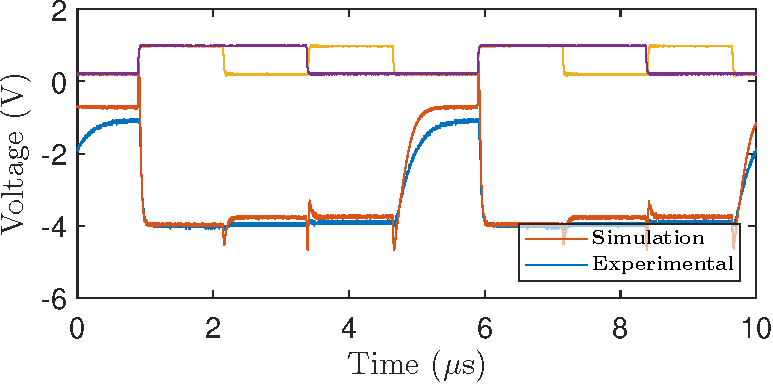
\includegraphics[width=1\linewidth, height = 5.1cm]{Appendices/NOR400K.pdf}
    \caption{Experimental and simulation NOR gate output voltage at 400 kHz Shifted by 1.5 V. The gate input voltages have been scaled and offset to the top of the diagram.}
    \label{fig:enter-label}
\end{figure}

\begin{figure}[h]
    \centering
    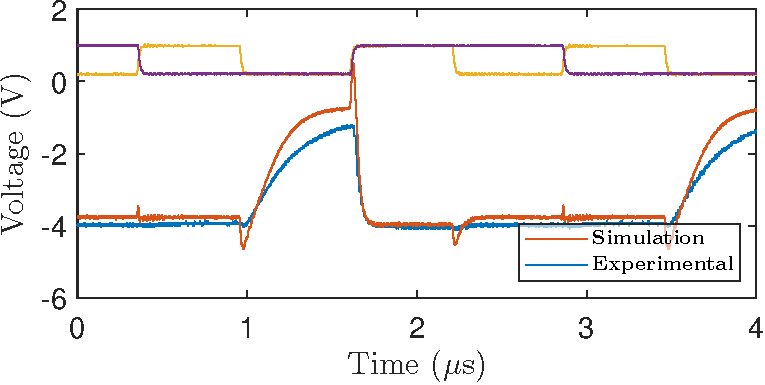
\includegraphics[width=1\linewidth, height = 5.1cm]{Images/NOR800K.pdf}
    \caption{Experimental and simulation NOR gate output voltage at 800 kHz Shifted by 1.5 V. The gate input voltages have been scaled and offset to the top of the diagram.}
    \label{fig:enter-label}
\end{figure}

\begin{figure}[h]
    \centering
    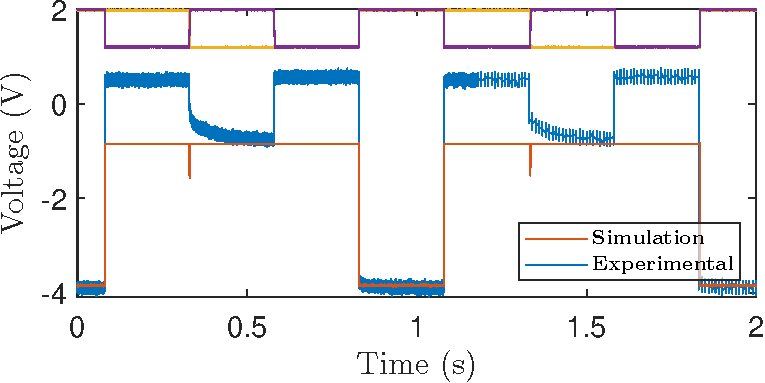
\includegraphics[width=1\linewidth, height = 5.1cm]{Appendices/NAND2.pdf}
    \caption{Experimental and simulation NAND gate output voltage at 2 Hz Shifted by 1.5 V. The gate input voltages have been scaled and offset to the top of the diagram.}
    \label{fig:enter-label}
\end{figure}

\begin{figure}[h]
    \centering
    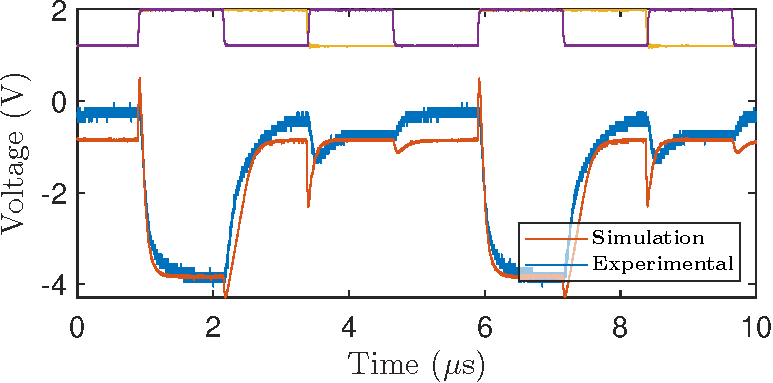
\includegraphics[width=1\linewidth, height = 5.1cm]{Appendices/NAND400K.pdf}
    \caption{Experimental and simulation NAND gate output voltage at 400 kHz Shifted by 2 V. The gate input voltages have been scaled and offset to the top of the diagram.}
    \label{fig:enter-label}
\end{figure}

\begin{figure}[h]
    \centering
    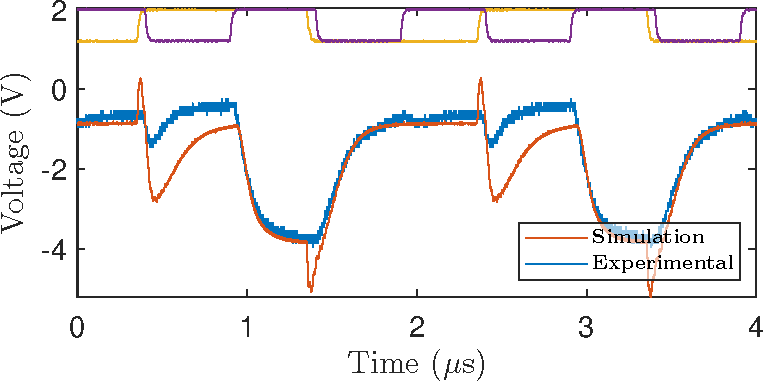
\includegraphics[width=1\linewidth, height = 5.1cm]{Images/NAND1000K.pdf}
    \caption{Experimental and simulation NAND gate output voltage at 1 MHz Shifted by 2 V. The gate input voltages have been scaled and offset to the top of the diagram.}
    \label{fig:enter-label}
\end{figure}